\documentclass[12pt]{article}

\title{CSC 455 - Assignment 5}
\author{Robert Krency}
\date{\today}

\usepackage{tikz}
\usepackage{amsmath}
\usepackage{graphicx}
\usepackage{tabularx}
\usepackage{multicol}
\usepackage{algpseudocode}
\usepackage{algorithm}
\usepackage{setspace}

% Include some source code
% https://tex.stackexchange.com/questions/348651/c-code-to-add-in-the-document
\usepackage{xcolor}
\usepackage{listings}

\definecolor{mGreen}{rgb}{0,0.6,0}
\definecolor{mGray}{rgb}{0.5,0.5,0.5}
\definecolor{mPurple}{rgb}{0.58,0,0.82}
\definecolor{backgroundColour}{rgb}{0.95,0.95,0.92}

\lstdefinestyle{CStyle}{
    backgroundcolor=\color{backgroundColour},   
    commentstyle=\color{mGreen},
    keywordstyle=\color{magenta},
    numberstyle=\tiny\color{mGray},
    stringstyle=\color{mPurple},
    basicstyle=\footnotesize,
    breakatwhitespace=false,         
    breaklines=true,                 
    captionpos=b,                    
    keepspaces=true,                 
    numbers=left,                    
    numbersep=5pt,                  
    showspaces=false,                
    showstringspaces=false,
    showtabs=false,                  
    tabsize=2,
    language=C
}

% Geometry 
\usepackage{geometry}
\geometry{letterpaper, left=20mm, top=20mm, right=20mm, bottom=20mm}

% Add vertical spacing to tables
\renewcommand{\arraystretch}{1.4}

\onehalfspacing

% Macros
\newcommand{\definition}[1]{\underline{\textbf{#1}}}

\newenvironment{rcases}
  {\left.\begin{aligned}}
  {\end{aligned}\right\rbrace}

% Begin Document
\begin{document}

\maketitle

\section{Two-Way Parameters}

The following C code was ran on a Windows 10 computer, compiled with GCC 10.3 using the MinGW project.

\begin{lstlisting}[style=CStyle]
    int* fun(int* a) {
        *a += 10;
        return a;
    }

    int main() {
        int a, b;
        a = 10;
        b = a + *fun(&a);
        printf("With the function call on the right,");
        printf(" b is: %d\n", b);

        a = 10;
        b = *fun(&a) + a;
        printf("With the function call on the left,");
        printf(" b is: %d\n", b);
    }
\end{lstlisting}

The purpose here is to determine when the parameter $a$ has its value fetched for the addition operation, and if there
is any difference in calling a function that modifies its value before or after the initial reference. 
The results are shown below:

\vspace{5mm}

\begin{center}
    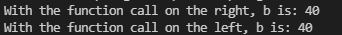
\includegraphics{a5-params.png}
\end{center}

As can be seen, the function $fun$ is ran prior to any operations taken place in the assignment statement of $b$.
For this configuration, there was no difference.
The variable $a$ was modified prior to the values being fetched for the addition operation.

\pagebreak

\section{Bonus}

The following C code was ran on a Windows 10 computer, compiled with GCC 10.3 using the MinGW project.

\begin{lstlisting}[style=CStyle]
    int x = 0;
    if (x == 0 && x++==1);
    printf("X is %d\n",x);
    if (x == 3 && x++==2);
    printf("X is %d\n", x);
\end{lstlisting}

The purpose here is to determine if short circuiting is happening inside the conditional statements.
The results are shown below:

\vspace{5mm}

\begin{center}
    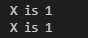
\includegraphics{a5-bonus.png}
\end{center}

As can be seen, the first conditional statement checked both input conditions, which resulted in the incrememnt of $x$ being executed in the first conditional.
However, as the $x == 3$ condition fails in the second conditional, the second increment of $x$ is never called.
This leads to the conclusion that short circuiting does indeed happen.

\end{document}

